% fig15 — Antal–Krapivsky vs this paper: shared branching skeleton, different observables
% Conceptual figure for §5.6 / introduction trap paragraph.
% Rebuild: pdflatex fig15_ak_contrast.tex  (from this directory)
\documentclass[tikz,border=14pt]{standalone}
\usepackage{amsmath,amssymb}
\usepackage{xcolor}
\usepackage{tikz}
\usetikzlibrary{
  arrows.meta,
  calc,
  positioning,
  backgrounds,
  fit
}

% Palette (SHARED_CONVENTIONS / TT visualiser)
\definecolor{type1}{HTML}{0072B2}
\definecolor{type2}{HTML}{D55E00}
\definecolor{ink}{HTML}{1a1c1f}
\definecolor{inksoft}{HTML}{565b62}
\definecolor{catred}{HTML}{9a2820}
\definecolor{type1fill}{HTML}{E8F4FA}
\definecolor{type2fill}{HTML}{FDF0E6}
\definecolor{catfill}{HTML}{F8EBE9}

\tikzset{
  >=Latex,
  every node/.style={font=\sffamily\small, text=ink},
  paneltitle/.style={
    font=\sffamily\bfseries\large,
    text=ink,
    align=center
  },
  sinkbox/.style={
    rounded corners=5pt,
    draw=catred,
    fill=catfill,
    line width=1.15pt,
    align=center,
    minimum width=2.85cm,
    minimum height=1.05cm,
    inner sep=4pt
  },
  typechip/.style={
    rounded corners=4pt,
    line width=1.05pt,
    align=center,
    minimum width=1.55cm,
    minimum height=0.88cm,
    inner sep=3pt,
    font=\sffamily\footnotesize
  },
  type1chip/.style={typechip, draw=type1, fill=type1fill},
  type2chip/.style={typechip, draw=type2, fill=type2fill},
  arr/.style={-{Latex[length=2.2mm,width=1.55mm]}, line width=1.0pt, draw=inksoft},
  arrcat/.style={-{Latex[length=2.2mm,width=1.55mm]}, line width=1.1pt, draw=catred},
}

\begin{document}
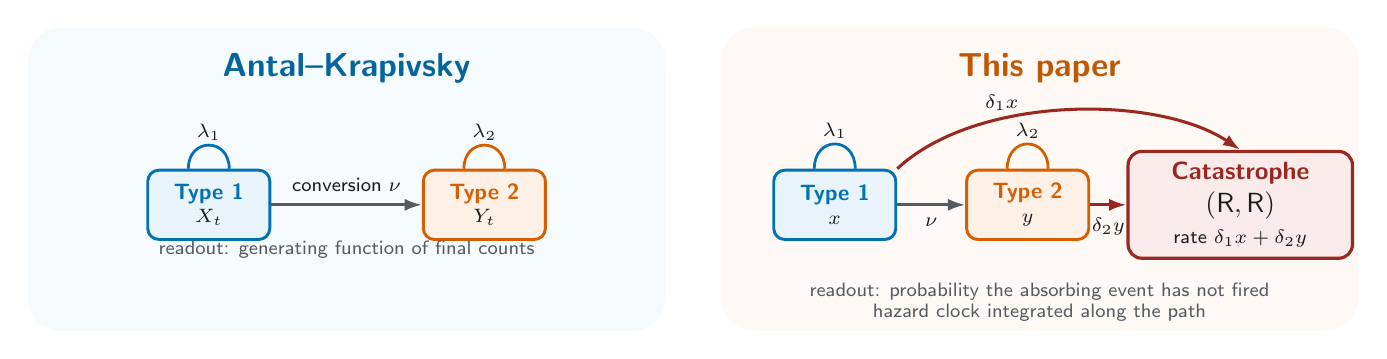
\begin{tikzpicture}[x=1cm, y=1cm]

  % =====================================================================
  % LEFT PANEL — Antal–Krapivsky
  % =====================================================================
  \begin{scope}[on background layer]
    \fill[type1fill!42, rounded corners=12pt]
      (0.15, 4.55) rectangle (8.25, 8.40);
  \end{scope}

  \node[paneltitle, anchor=north, text=type1!85!ink]
    at (4.2, 8.20) {Antal--Krapivsky};

  % Mini process (counts only)
  \node[type1chip] (Lt1) at (2.45, 6.15) {%
    {\color{type1}\bfseries Type 1}\\[-1pt]
    {\scriptsize $X_t$}
  };
  \node[type2chip] (Lt2) at (5.95, 6.15) {%
    {\color{type2}\bfseries Type 2}\\[-1pt]
    {\scriptsize $Y_t$}
  };
  \draw[arr] (Lt1) -- (Lt2)
    node[midway, above=1pt, font=\sffamily\scriptsize\color{inksoft}]
      {conversion $\nu$};
  \draw[type1, line width=1.0pt]
    ([xshift=-0.26cm]Lt1.north)
      .. controls ([xshift=-0.26cm,yshift=0.40cm]Lt1.north)
              and ([xshift= 0.26cm,yshift=0.40cm]Lt1.north) ..
    ([xshift= 0.26cm]Lt1.north)
    node[pos=0.5, above=-2pt, font=\sffamily\scriptsize\color{type1}] {$\lambda_1$};
  \draw[type2, line width=1.0pt]
    ([xshift=-0.26cm]Lt2.north)
      .. controls ([xshift=-0.26cm,yshift=0.40cm]Lt2.north)
              and ([xshift= 0.26cm,yshift=0.40cm]Lt2.north) ..
    ([xshift= 0.26cm]Lt2.north)
    node[pos=0.5, above=-2pt, font=\sffamily\scriptsize\color{type2}] {$\lambda_2$};

  \node[font=\sffamily\scriptsize, text=inksoft, align=center]
    at (4.2, 5.58)
    {readout: generating function of final counts};

  % =====================================================================
  % RIGHT PANEL — this paper
  % =====================================================================
  \begin{scope}[on background layer]
    \fill[type2fill!40, rounded corners=12pt]
      (8.95, 4.55) rectangle (17.05, 8.40);
  \end{scope}

  \node[paneltitle, anchor=north, text=type2!90!ink]
    at (13.0, 8.20) {This paper};

  % Type chips + catastrophe sink (horizontal)
  \node[type1chip] (Rt1) at (10.40, 6.15) {%
    {\color{type1}\bfseries Type 1}\\[-1pt]
    {\scriptsize $x$}
  };
  \node[type2chip] (Rt2) at (12.85, 6.15) {%
    {\color{type2}\bfseries Type 2}\\[-1pt]
    {\scriptsize $y$}
  };
  \node[sinkbox] (Rcat) at (15.55, 6.15) {%
    {\color{catred}\sffamily\bfseries Catastrophe}\\[1pt]
    {\normalsize$(\mathsf{R},\mathsf{R})$}\\[0pt]
    {\sffamily\scriptsize rate $\delta_1 x+\delta_2 y$}
  };

  \draw[arr] (Rt1) -- (Rt2)
    node[midway, below=1pt, font=\sffamily\scriptsize\color{inksoft}]
      {$\nu$};

  % Birth loops (short; labels inside loops to avoid collision with hazard arc)
  \draw[type1, line width=1.0pt]
    ([xshift=-0.26cm]Rt1.north)
      .. controls ([xshift=-0.26cm,yshift=0.42cm]Rt1.north)
              and ([xshift= 0.26cm,yshift=0.42cm]Rt1.north) ..
    ([xshift= 0.26cm]Rt1.north)
    node[pos=0.5, above=-2pt, font=\sffamily\scriptsize\color{type1}] {$\lambda_1$};
  \draw[type2, line width=1.0pt]
    ([xshift=-0.26cm]Rt2.north)
      .. controls ([xshift=-0.26cm,yshift=0.42cm]Rt2.north)
              and ([xshift= 0.26cm,yshift=0.42cm]Rt2.north) ..
    ([xshift= 0.26cm]Rt2.north)
    node[pos=0.5, above=-2pt, font=\sffamily\scriptsize\color{type2}] {$\lambda_2$};

  % Hazard arcs high enough to clear birth-loop labels
  \draw[arrcat]
    (Rt1.north east)
      .. controls (12.2, 7.55) and (14.5, 7.55) ..
    (Rcat.north)
    node[pos=0.33, above=-1pt, font=\sffamily\scriptsize\color{catred}] {$\delta_1 x$};
  \draw[arrcat]
    (Rt2.east) -- (Rcat.west)
    node[midway, below=1pt, font=\sffamily\scriptsize\color{catred}] {$\delta_2 y$};

  \node[font=\sffamily\scriptsize, text=inksoft, align=center]
    at (13.0, 5.05)
    {readout: probability the absorbing event has not fired};

  \node[font=\sffamily\scriptsize, text=inksoft, align=center]
    at (13.0, 4.78)
    {hazard clock integrated along the path};

\end{tikzpicture}
\end{document}
